
%% bare_conf.tex
%% V1.3
%% 2007/01/11
%% by Michael Shell
%% See:
%% http://www.michaelshell.org/
%% for current contact information.
%%
%% This is a skeleton file demonstrating the use of IEEEtran.cls
%% (requires IEEEtran.cls version 1.7 or later) with an IEEE conference paper.
%%
%% Support sites:
%% http://www.michaelshell.org/tex/ieeetran/
%% http://www.ctan.org/tex-archive/macros/latex/contrib/IEEEtran/
%% and
%% http://www.ieee.org/

%%*************************************************************************
%% Legal Notice:
%% This code is offered as-is without any warranty either expressed or
%% implied; without even the implied warranty of MERCHANTABILITY or
%% FITNESS FOR A PARTICULAR PURPOSE! 
%% User assumes all risk.
%% In no event shall IEEE or any contributor to this code be liable for
%% any damages or losses, including, but not limited to, incidental,
%% consequential, or any other damages, resulting from the use or misuse
%% of any information contained here.
%%
%% All comments are the opinions of their respective authors and are not
%% necessarily endorsed by the IEEE.
%%
%% This work is distributed under the LaTeX Project Public License (LPPL)
%% ( http://www.latex-project.org/ ) version 1.3, and may be freely used,
%% distributed and modified. A copy of the LPPL, version 1.3, is included
%% in the base LaTeX documentation of all distributions of LaTeX released
%% 2003/12/01 or later.
%% Retain all contribution notices and credits.
%% ** Modified files should be clearly indicated as such, including  **
%% ** renaming them and changing author support contact information. **
%%
%% File list of work: IEEEtran.cls, IEEEtran_HOWTO.pdf, bare_adv.tex,
%%                    bare_conf.tex, bare_jrnl.tex, bare_jrnl_compsoc.tex
%%*************************************************************************

% *** Authors should verify (and, if needed, correct) their LaTeX system  ***
% *** with the testflow diagnostic prior to trusting their LaTeX platform ***
% *** with production work. IEEE's font choices can trigger bugs that do  ***
% *** not appear when using other class files.                            ***
% The testflow support page is at:
% http://www.michaelshell.org/tex/testflow/



% Note that the a4paper option is mainly intended so that authors in
% countries using A4 can easily print to A4 and see how their papers will
% look in print - the typesetting of the document will not typically be
% affected with changes in paper size (but the bottom and side margins will).
% Use the testflow package mentioned above to verify correct handling of
% both paper sizes by the user's LaTeX system.
%
% Also note that the "draftcls" or "draftclsnofoot", not "draft", option
% should be used if it is desired that the figures are to be displayed in
% draft mode.
%
\documentclass[10pt, conference, compsocconf]{IEEEtran}
% Add the compsocconf option for Computer Society conferences.
%
% If IEEEtran.cls has not been installed into the LaTeX system files,
% manually specify the path to it like:
% \documentclass[conference]{../sty/IEEEtran}





% Some very useful LaTeX packages include:
% (uncomment the ones you want to load)


% *** MISC UTILITY PACKAGES ***
%
%\usepackage{ifpdf}
% Heiko Oberdiek's ifpdf.sty is very useful if you need conditional
% compilation based on whether the output is pdf or dvi.
% usage:
% \ifpdf
%   % pdf code
% \else
%   % dvi code
% \fi
% The latest version of ifpdf.sty can be obtained from:
% http://www.ctan.org/tex-archive/macros/latex/contrib/oberdiek/
% Also, note that IEEEtran.cls V1.7 and later provides a builtin
% \ifCLASSINFOpdf conditional that works the same way.
% When switching from latex to pdflatex and vice-versa, the compiler may
% have to be run twice to clear warning/error messages.






% *** CITATION PACKAGES ***
%
%\usepackage{cite}
% cite.sty was written by Donald Arseneau
% V1.6 and later of IEEEtran pre-defines the format of the cite.sty package
% \cite{} output to follow that of IEEE. Loading the cite package will
% result in citation numbers being automatically sorted and properly
% "compressed/ranged". e.g., [1], [9], [2], [7], [5], [6] without using
% cite.sty will become [1], [2], [5]--[7], [9] using cite.sty. cite.sty's
% \cite will automatically add leading space, if needed. Use cite.sty's
% noadjust option (cite.sty V3.8 and later) if you want to turn this off.
% cite.sty is already installed on most LaTeX systems. Be sure and use
% version 4.0 (2003-05-27) and later if using hyperref.sty. cite.sty does
% not currently provide for hyperlinked citations.
% The latest version can be obtained at:
% http://www.ctan.org/tex-archive/macros/latex/contrib/cite/
% The documentation is contained in the cite.sty file itself.






% *** GRAPHICS RELATED PACKAGES ***
%
\ifCLASSINFOpdf
  % \usepackage[pdftex]{graphicx}
  % declare the path(s) where your graphic files are
  % \graphicspath{{../pdf/}{../jpeg/}}
  % and their extensions so you won't have to specify these with
  % every instance of \includegraphics
  % \DeclareGraphicsExtensions{.pdf,.jpeg,.png}
\else
  % or other class option (dvipsone, dvipdf, if not using dvips). graphicx
  % will default to the driver specified in the system graphics.cfg if no
  % driver is specified.
  % \usepackage[dvips]{graphicx}
  % declare the path(s) where your graphic files are
  % \graphicspath{{../eps/}}
  % and their extensions so you won't have to specify these with
  % every instance of \includegraphics
  % \DeclareGraphicsExtensions{.eps}
\fi
% graphicx was written by David Carlisle and Sebastian Rahtz. It is
% required if you want graphics, photos, etc. graphicx.sty is already
% installed on most LaTeX systems. The latest version and documentation can
% be obtained at: 
% http://www.ctan.org/tex-archive/macros/latex/required/graphics/
% Another good source of documentation is "Using Imported Graphics in
% LaTeX2e" by Keith Reckdahl which can be found as epslatex.ps or
% epslatex.pdf at: http://www.ctan.org/tex-archive/info/
%
% latex, and pdflatex in dvi mode, support graphics in encapsulated
% postscript (.eps) format. pdflatex in pdf mode supports graphics
% in .pdf, .jpeg, .png and .mps (metapost) formats. Users should ensure
% that all non-photo figures use a vector format (.eps, .pdf, .mps) and
% not a bitmapped formats (.jpeg, .png). IEEE frowns on bitmapped formats
% which can result in "jaggedy"/blurry rendering of lines and letters as
% well as large increases in file sizes.
%
% You can find documentation about the pdfTeX application at:
% http://www.tug.org/applications/pdftex





% *** MATH PACKAGES ***
%
%\usepackage[cmex10]{amsmath}
% A popular package from the American Mathematical Society that provides
% many useful and powerful commands for dealing with mathematics. If using
% it, be sure to load this package with the cmex10 option to ensure that
% only type 1 fonts will utilized at all point sizes. Without this option,
% it is possible that some math symbols, particularly those within
% footnotes, will be rendered in bitmap form which will result in a
% document that can not be IEEE Xplore compliant!
%
% Also, note that the amsmath package sets \interdisplaylinepenalty to 10000
% thus preventing page breaks from occurring within multiline equations. Use:
%\interdisplaylinepenalty=2500
% after loading amsmath to restore such page breaks as IEEEtran.cls normally
% does. amsmath.sty is already installed on most LaTeX systems. The latest
% version and documentation can be obtained at:
% http://www.ctan.org/tex-archive/macros/latex/required/amslatex/math/

% Include other packages here, before hyperref.
\usepackage{graphicx}
\usepackage{amsmath}
\usepackage{amssymb}
\usepackage{booktabs}

% *** SPECIALIZED LIST PACKAGES ***
%
%\usepackage{algorithmic}
% algorithmic.sty was written by Peter Williams and Rogerio Brito.
% This package provides an algorithmic environment fo describing algorithms.
% You can use the algorithmic environment in-text or within a figure
% environment to provide for a floating algorithm. Do NOT use the algorithm
% floating environment provided by algorithm.sty (by the same authors) or
% algorithm2e.sty (by Christophe Fiorio) as IEEE does not use dedicated
% algorithm float types and packages that provide these will not provide
% correct IEEE style captions. The latest version and documentation of
% algorithmic.sty can be obtained at:
% http://www.ctan.org/tex-archive/macros/latex/contrib/algorithms/
% There is also a support site at:
% http://algorithms.berlios.de/index.html
% Also of interest may be the (relatively newer and more customizable)
% algorithmicx.sty package by Szasz Janos:
% http://www.ctan.org/tex-archive/macros/latex/contrib/algorithmicx/




% *** ALIGNMENT PACKAGES ***
%
%\usepackage{array}
% Frank Mittelbach's and David Carlisle's array.sty patches and improves
% the standard LaTeX2e array and tabular environments to provide better
% appearance and additional user controls. As the default LaTeX2e table
% generation code is lacking to the point of almost being broken with
% respect to the quality of the end results, all users are strongly
% advised to use an enhanced (at the very least that provided by array.sty)
% set of table tools. array.sty is already installed on most systems. The
% latest version and documentation can be obtained at:
% http://www.ctan.org/tex-archive/macros/latex/required/tools/


%\usepackage{mdwmath}
%\usepackage{mdwtab}
% Also highly recommended is Mark Wooding's extremely powerful MDW tools,
% especially mdwmath.sty and mdwtab.sty which are used to format equations
% and tables, respectively. The MDWtools set is already installed on most
% LaTeX systems. The lastest version and documentation is available at:
% http://www.ctan.org/tex-archive/macros/latex/contrib/mdwtools/


% IEEEtran contains the IEEEeqnarray family of commands that can be used to
% generate multiline equations as well as matrices, tables, etc., of high
% quality.


%\usepackage{eqparbox}
% Also of notable interest is Scott Pakin's eqparbox package for creating
% (automatically sized) equal width boxes - aka "natural width parboxes".
% Available at:
% http://www.ctan.org/tex-archive/macros/latex/contrib/eqparbox/





% *** SUBFIGURE PACKAGES ***
%\usepackage[tight,footnotesize]{subfigure}
% subfigure.sty was written by Steven Douglas Cochran. This package makes it
% easy to put subfigures in your figures. e.g., "Figure 1a and 1b". For IEEE
% work, it is a good idea to load it with the tight package option to reduce
% the amount of white space around the subfigures. subfigure.sty is already
% installed on most LaTeX systems. The latest version and documentation can
% be obtained at:
% http://www.ctan.org/tex-archive/obsolete/macros/latex/contrib/subfigure/
% subfigure.sty has been superceeded by subfig.sty.



%\usepackage[caption=false]{caption}
%\usepackage[font=footnotesize]{subfig}
% subfig.sty, also written by Steven Douglas Cochran, is the modern
% replacement for subfigure.sty. However, subfig.sty requires and
% automatically loads Axel Sommerfeldt's caption.sty which will override
% IEEEtran.cls handling of captions and this will result in nonIEEE style
% figure/table captions. To prevent this problem, be sure and preload
% caption.sty with its "caption=false" package option. This is will preserve
% IEEEtran.cls handing of captions. Version 1.3 (2005/06/28) and later 
% (recommended due to many improvements over 1.2) of subfig.sty supports
% the caption=false option directly:
%\usepackage[caption=false,font=footnotesize]{subfig}
%
% The latest version and documentation can be obtained at:
% http://www.ctan.org/tex-archive/macros/latex/contrib/subfig/
% The latest version and documentation of caption.sty can be obtained at:
% http://www.ctan.org/tex-archive/macros/latex/contrib/caption/




% *** FLOAT PACKAGES ***
%
%\usepackage{fixltx2e}
% fixltx2e, the successor to the earlier fix2col.sty, was written by
% Frank Mittelbach and David Carlisle. This package corrects a few problems
% in the LaTeX2e kernel, the most notable of which is that in current
% LaTeX2e releases, the ordering of single and double column floats is not
% guaranteed to be preserved. Thus, an unpatched LaTeX2e can allow a
% single column figure to be placed prior to an earlier double column
% figure. The latest version and documentation can be found at:
% http://www.ctan.org/tex-archive/macros/latex/base/



%\usepackage{stfloats}
% stfloats.sty was written by Sigitas Tolusis. This package gives LaTeX2e
% the ability to do double column floats at the bottom of the page as well
% as the top. (e.g., "\begin{figure*}[!b]" is not normally possible in
% LaTeX2e). It also provides a command:
%\fnbelowfloat
% to enable the placement of footnotes below bottom floats (the standard
% LaTeX2e kernel puts them above bottom floats). This is an invasive package
% which rewrites many portions of the LaTeX2e float routines. It may not work
% with other packages that modify the LaTeX2e float routines. The latest
% version and documentation can be obtained at:
% http://www.ctan.org/tex-archive/macros/latex/contrib/sttools/
% Documentation is contained in the stfloats.sty comments as well as in the
% presfull.pdf file. Do not use the stfloats baselinefloat ability as IEEE
% does not allow \baselineskip to stretch. Authors submitting work to the
% IEEE should note that IEEE rarely uses double column equations and
% that authors should try to avoid such use. Do not be tempted to use the
% cuted.sty or midfloat.sty packages (also by Sigitas Tolusis) as IEEE does
% not format its papers in such ways.





% *** PDF, URL AND HYPERLINK PACKAGES ***
%
%\usepackage{url}
% url.sty was written by Donald Arseneau. It provides better support for
% handling and breaking URLs. url.sty is already installed on most LaTeX
% systems. The latest version can be obtained at:
% http://www.ctan.org/tex-archive/macros/latex/contrib/misc/
% Read the url.sty source comments for usage information. Basically,
% \url{my_url_here}.

\usepackage[pdftex]{hyperref}



% *** Do not adjust lengths that control margins, column widths, etc. ***
% *** Do not use packages that alter fonts (such as pslatex).         ***
% There should be no need to do such things with IEEEtran.cls V1.6 and later.
% (Unless specifically asked to do so by the journal or conference you plan
% to submit to, of course. )


% correct bad hyphenation here
\hyphenation{op-tical net-works semi-conduc-tor}


\begin{document}
%
% paper title
% can use linebreaks \\ within to get better formatting as desired
\title{Aplicação de métodos de aprendizado de máquina para predição de desfecho clínico}


% author names and affiliations
% use a multiple column layout for up to two different
% affiliations

\author{\IEEEauthorblockN{Guilherme Silva de Camargo}
\IEEEauthorblockA{Departamento de computação (DComp)\\
Universidade Federal de São Carlos (UFSCar)\\
18052-780, Sorocaba, São Paulo, Brasil\\
guilhermecamargo@estudante.ufscar.br}
}

% conference papers do not typically use \thanks and this command
% is locked out in conference mode. If really needed, such as for
% the acknowledgment of grants, issue a \IEEEoverridecommandlockouts
% after \documentclass

% for over three affiliations, or if they all won't fit within the width
% of the page, use this alternative format:
% 
%\author{\IEEEauthorblockN{Michael Shell\IEEEauthorrefmark{1},
%Homer Simpson\IEEEauthorrefmark{2},
%James Kirk\IEEEauthorrefmark{3}, 
%Montgomery Scott\IEEEauthorrefmark{3} and
%Eldon Tyrell\IEEEauthorrefmark{4}}
%\IEEEauthorblockA{\IEEEauthorrefmark{1}School of Electrical and Computer Engineering\\
%Georgia Institute of Technology,
%Atlanta, Georgia 30332--0250\\ Email: see http://www.michaelshell.org/contact.html}
%\IEEEauthorblockA{\IEEEauthorrefmark{2}Twentieth Century Fox, Springfield, USA\\
%Email: homer@thesimpsons.com}
%\IEEEauthorblockA{\IEEEauthorrefmark{3}Starfleet Academy, San Francisco, California 96678-2391\\
%Telephone: (800) 555--1212, Fax: (888) 555--1212}
%\IEEEauthorblockA{\IEEEauthorrefmark{4}Tyrell Inc., 123 Replicant Street, Los Angeles, California 90210--4321}}




% use for special paper notices
%\IEEEspecialpapernotice{(Invited Paper)}




% make the title area
\maketitle


\begin{abstract}
A leucemia é um tipo de tumor que afeta a médula óssea, dessa forma, na leucemia mieloide aguda, as células-tronco mieloides, que originam as células sanguíneas, sofrem algumas mutações genéticas, cujo o entendimento sobre a relação entre os genes causadores, e outros dados ainda não é totalmente conhecida . Nesse sentido, este trabalho visa entender através dessas informações (expressão genética, mutações gênicas e dados clínicos) uma relação entre esses dados, para conseguir obter uma predição de desfecho clínico, indicando a probabilidade do tratamento resultar em óbito do paciente, ou sobrevivência. Com isso, identificando melhores combinações de tratamentos, adaptadas aos dados de cada paciente, tal como idade do mesmo, auxiliando na escolha do tratatamento mais indicado para cada paciente. Por fim, foi obtido resultados de por volta de 75\% de acerto na predição, utilizando os métodos de classificação Regressão Logistica e Rede Neural Artificial (Perceptron multicamada) mostrando ser mais uma útil ferramenta no âmbito de auxiliar a escolha do tratamento, ou a diminuição da imaterialidade na relação entre os dados clínicos, e géneticos do paciente, sendo promisssor para estudos ainda mais aprofundados.

\end{abstract}

\begin{IEEEkeywords}
aprendizado de máquina, leucemia mieloide aguda; predição clínica.

\end{IEEEkeywords}


% For peer review papers, you can put extra information on the cover
% page as needed:
% \ifCLASSOPTIONpeerreview
% \begin{center} \bfseries EDICS Category: 3-BBND \end{center}
% \fi
%
% For peerreview papers, this IEEEtran command inserts a page break and
% creates the second title. It will be ignored for other modes.
\IEEEpeerreviewmaketitle



\section{Introdução}
\label{sec:intro}
A leucemia mielóide aguda (LMA) é uma doença rara que afeta a medula óssea, as células-tronco dos pacientes com essa doença sofrem uma mutação genética. As células sanguíneas são formadas a partir dessas células-tronco, consistindo de leucócitos, glóbulos vermelhos e plaquetas. Nessa situação, as células ficam doentes, incapazes de se desenvolver e começam a se multiplicar descontroladamente. Há incerteza nos fatores diretos causadores da doença, por isso a relação entre os dados clínicos e genéticos com o nível que a doença apresenta não é sabido com precisão. 

Por isso, na maioria dos casos o médico vale-se de estudos para predizer o tratamento, tal como as recomendações para diagnóstico e tratamento publicados pelo grupo de pesquisa European LeukemiaNet (ELN), atualizado pela última vez em 2022, porém mesmo esses estudos, não levam em consideração dados como a idade do paciente, o qual são valiosos para determinar um tratamento ao paciente, assim, as respostas terapêuticas a tratamentos por parte dos pacientes mesmo classificados como pertencentes ao mesmo grupo pelo ELN, podem apresentar diferenças, como por exemplo, a reação diferente a um mesmo medicamento.

Dessa forma, mostra-se muito valioso apresentar mais uma alternativa para ajudar na predição da chance de sobrevivência dos pacientes dado o conjunto de dados clínico e o tratamento prescrito, nesse sentido, este trabalho propõe um sistema para auxiliar o médico na prescrição do tratamento médico, dado as características de cada caso, através da predição de desfecho clínico, predizendo a probabilidade de sobrevivência e óbito mediante os dados clínicos e genéticos do paciente, visto que a área de aprendizado de máquina com suas diversas técnicas vêm mostrando-se eficaz no encontro de padrões e relações em grandes volumes de dados.

Com isso, é esperado reduzir a abstração e subjetividade na predição de tratamentos médicos no contexto da LMA, aumentando a assertividade na indicação de tratamentos aos pacientes, ocasionando um aumento da sobrevida e qualidade de vida para estes pacientes. 

\section{Dados e pré-processamento}
\label{sec:formatting}
A base de dados conta com três diferentes tipos de informações, dados clínicos, de expressão genética e de mutação gênica, inicialmente a base com dados clínicos continha 390 amostras com 10 atributos; expressão genética com 304 amostras e 14712 atributos; e mutação gênica com 362 amostras e 318 atributos. Porém, estas bases continham atributos com valores faltantes, amostras duplicadas e valores categóricos em alguns atributos.

No entanto, é importante entender quais são os atributos, e seu significado, nesse sentido, os 10 atributos clínicos são: “Diagnosis Age”, idade de diagnóstico; “Bone Marrow Blast Percentage”, porcentagem de blastos na medula óssea do paciente; “Mutation Count”, contador de mutações gênicas no paciente; “PB Blast Percentage”, porcentagem de blastos em sangue periférico do paciente; “WBC”, leucócitos no sangue do paciente; “Sex”, sexo do paciente; “Race”, raça do paciente; “Cytogenetic Info”, informações citogenéticas do paciente; “ELN Risk Classification", classificação de risco molecular do paciente; e “Treatment Intensity”, intensidade do tratamento.  

Ademais, a base de dados contendo as expressões genéticas têm diversos atributos, sendo cada um gene diferente, representado por um valor numérico, que busca expressar o quanto aquele gene está presente no paciente, que pode ser definido como o processo pelo qual a informação hereditária contida em um gene, como uma sequência de DNA, é usada para produzir um produto gênico funcional, como proteínas ou RNA.

Por fim, o mesmo ocorre com as mutações gênicas, tendo diversos atributos, também sendo um gene diferente representado por cada atributo, mas diferente na representação, visto que o valor contido é representado por 0, ausência de mutação no gene e 1 demonstrado que aquele gene sofreu mutação.

\subsection{Análise de dados}
Para definir os pré-processamentos foi utilizado diversos gráficos e medidas descritivas utilizando os 10 atributos descritos dos dados clínicos, sendo estes box plots, gráficos de barras para os valores médios dos atributos, histogramas e gráficos de dispersão, além disso, tivemos medidas como a média, desvio padrão, quantidade, mínimo, máximo, mediana, 1° e 3°quartil, e as matrizes de covariância e correlação.

Nesse contexto, será explicitada apenas as informações que impactam diretamente na escolha dos pré-processamentos, e mais a frente na seleção dos atributos. Dessa forma, pode-se identificar através dos box plots que a distribuição da classe “Overall Survival Status", está bem distinta para seus dois valores, no boxplot dos atributos “Diagnosis Age” e “ELN Risk Classification”, assim, indicando que as duas classes têm distribuições significativamente diferentes, como pode ser visto na figura 1, porém isso não ocorre para os outros atributos.

Ademais, utilizando os gráficos de dispersão foi possível identificar que para os valores acima de 60 anos do atributo “Diagnosis Age” há predominância da classe 1, como pode ser constatado na figura 2.

Por fim, com o histograma para raça foi possível identificar os diferentes valores para o atributo, a fim de agrupá-los posteriormente.

\begin{figure}
  \centering
  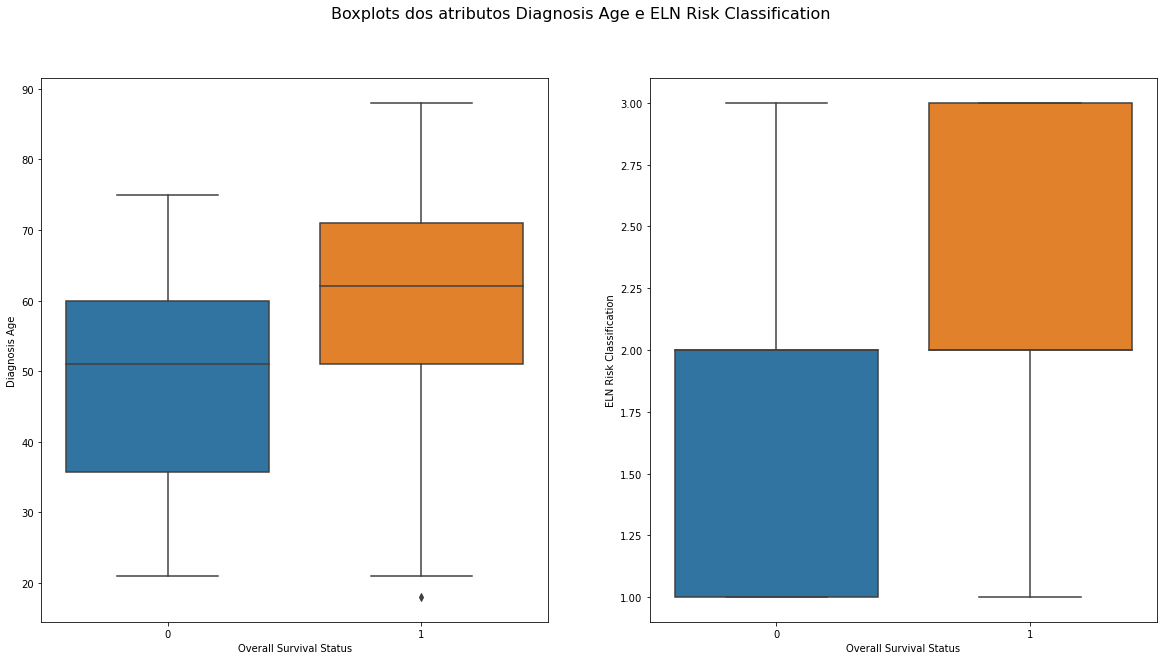
\includegraphics[width=.40\textwidth]{boxplots.png}
  \caption{Box plots para os atributos clínicos}
\label{fig:short}
\end{figure}

\begin{figure}
  \centering
  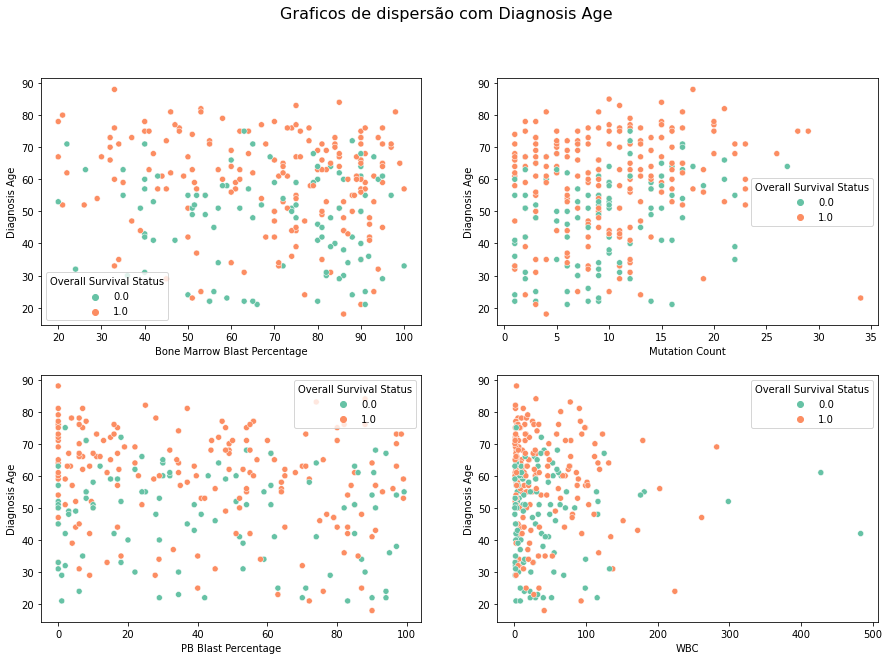
\includegraphics[width=.40\textwidth]{disp.png}
  \caption{Gráficos de dispersão para os atributos clínicos}
\label{fig:short}
\end{figure}

\subsection{Pré-Processamentos}
Como visto anteriormente nas análises feitas, temos dados faltantes, nesse sentido, temos o primeiro pré-processamento ao qual foi utilizado a média dos atributos para substituir esses valores. Além da média, tivemos testes com a mediana, mas essa não representou grandes ganhos, tendo desempenhos piores que a média. Assim, optou-se pela média, escolha inicial que deu-se pelos seguintes fatores, manutenção da estrutura de dados, a média ajuda a manter a estrutura dos dados originais, melhoria da precisão de análises estatísticas, pois é um bom estimador do valor verdadeiro quando os dados estão distribuídos e redução da perda de informação.

Ademais, os atributos categóricos foram convertidos em vários atributos com valores de 0 para não está presente, e 1 indicando que está presente naquela amostra. Além disso, tivemos as raças sendo agrupadas, já que havia diferentes valores em formato de texto que continham a mesma informação, pois estavam escritos com letras maiúsculas em um dos casos e minúsculas em outros, assim, estavam representados como valores diferentes, o que não seria o caso, como por exemplo “White” e “WHITE”.

Por fim, temos a tabela I, indicando a quantidade de amostras e atributos para cada base de dados após os pré-processamentos. 

\begin{table}[]
\caption{Quantidade de amostras e atributos nas bases}
\centering
\resizebox{\columnwidth}{!}{%
\begin{tabular}{|c|c|c|}
\hline
Base de dados & Amostras (Treino/Teste) & Atributos\\ \hline
Clínica      & 316 / 28      & 38\\ \hline
Expressão genética & 316 / 28 & 14713\\ \hline
Mutação gênica     & 316 / 28 & 319\\ \hline
\end{tabular}%
}
\end{table}

\section{Protocolo experimental}
Inicialmente, após a realização dos pré-processamentos, agrupou-se todos as três bases de dados para realizar os primeiros experimentos, foram testados os seguintes algoritmos de classificação, k-vizinhos mais próximos (KNN), Naive Bayes Gaussiano, Regressão Logística, Rede Neural Artificial (Perceptron multicamada), Máquina de Vetores de Suporte e Floresta Aleatória. Assim, os primeiros resultados com a base toda podem ser vistos na tabela II.

Além disso, como será explicitado nos próximos tópicos, para buscar o melhor desempenho, e uma maior generalização dos modelos, utilizando diversas métricas, houve seleção dos melhores atributos para cada base de dados. Dessa forma, obteve-se resultados melhores, aos quais serão explicados na sequência. 

\begin{table}[]
\caption{Métricas dos algoritmos com a base completa}
\centering
\resizebox{\columnwidth}{!}{%
\begin{tabular}{|c|c|c|c|c|c|}
\hline
Classificador & Acurácia & Desvio Padrão & Curva ROC & F1\\ \hline
KNN           & 0.622    & 0.105         & 0.540     & 0.736\\ \hline
Naive Bayes   & 0.467    & 0.103         & 0.519     & 0.344\\ \hline
Regressão Logistica & 0.679 & 0.076 & 0.621 & 0.760\\ \hline
Rede Neural Artificial & 0.590 & 0.118 & 0.544 & 0.660\\ \hline
Máquina de Vetores de Suporte & 0.657 & 0.101 & 0.541 & 0.776\\ \hline
Floresta Aleatoria & 0.654 & 0.090 & 0.576 & 0.745\\ \hline
\end{tabular}%
}
\end{table}

\subsection{Descrição da forma de avaliação}
No treinamento dos métodos de classificação para a seleção de atributos, e na sequência para visualização do desempenho dos atributos escolhidos nos diversos métodos de classificação, utilizou-se o uso da técnica de validação cruzada com 10 folds, também conhecida como "cross-fold validation", esta técnica será particularmente útil, pois o conjunto de dados disponível é pequeno e precisa ser dividido em conjuntos de treinamento e teste para a avaliação do modelo, o que ajuda a garantir que o modelo não esteja super ajustando ou sub ajustando, assim, sendo mais fácil avaliar a capacidade de generalização dos modelos.

Ademais, após a seleção de atributos citada anteriormente, no treinamento dos métodos para a análise de resultados, geração de gráficos, matrizes e curvas, os dados foram divididos em 80\% para treinamento e 20\% para teste. 

Por fim, para predição dos dados de teste submetidos no Kaggle utilizou-se a base de dados completa.

\subsection{Medidas de desempenho empregadas}
Para avaliar os modelos, a princípio utilizou-se as métricas: Acurácia, proporção de exemplos classificados corretamente em relação ao número total de exemplos; Desvio Padrão, mede a variabilidade dos dados em relação à média; Curva ROC, avalia o desempenho de um modelo binário à medida que o limiar de classificação é variado;  Recall, mede a proporção de exemplos positivos que são classificados corretamente como positivos; Precisão, mede a proporção de exemplos classificados corretamente como positivos em relação ao número total de exemplos classificados como positivos; F1-score, medida de precisão e recall combinadas, calculada como a média harmônica dessas duas medidas. 

Porém, na avaliação dos resultados também utilizou-se curva de aprendizado, mostra a evolução do desempenho do modelo à medida que o tamanho do conjunto de treinamento é aumentado; e curva de validação, avalia o desempenho do modelo em diferentes hiperparâmetros.

\subsection{Ajuste de Parâmetros}
Como citado anteriormente, para buscar o melhor desempenho possível e uma melhor generalização dos dados, utilizou-se “seleção de features”, consiste em selecionar as k melhores features baseado nas pontuações mais altas, para calcular essas pontuações, utilizou-se nas bases contendo os dados clínicos e os dados de expressão genética o valor ANOVA (Análise de variância), e para a base contendo as mutações gênicas abordou-se o valor de estatísticas de qui-quadrado. 

Dessa forma, testou-se diversas combinações de k para as três bases de dados separadamente, agrupando os dados na sequência para treinando com o classificador de Regressão Logística, método ao qual apresentou melhor desempenho inicial, assim, selecionando os valores de k que obtiveram maior valor de curva ROC. Ademais, os diversos resultados das métricas para os diferentes valores de k, estão \href{https://drive.google.com/drive/folders/1tm04wXXDOEbq36WOWo67gdHbZM_52TB1?usp=sharing}{disponíveis neste link}.

Por fim, também testou-se ajustes de parâmetros para cada algoritmo, avaliando o desempenho de cada parâmetro também através da curva ROC.

\section{Resultados}
Inicialmente, após as seleções de atributos realizadas, pode-se perceber um grande ganho em todos as medidas, como por exemplo, obteve-se 72\% em média de acurácia dos algoritmos, demonstrado na tabela III, um ganho expressivo aos valores iniciais, demonstrados na tabela II. 

\begin{table}[]
\caption{Métricas dos algoritmos para a base com 72 atributos}
\centering
\resizebox{\columnwidth}{!}{%
\begin{tabular}{|c|c|c|c|c|c|}
\hline
Classificador & Acurácia & Desvio Padrão & Curva ROC & F1\\ \hline
KNN           & 0.711    & 0.075         & 0.630     & 0.801\\ \hline
Naive Bayes   & 0.714    & 0.074         & 0.629     & 0.799\\ \hline
Regressão Logistica & 0.731 & 0.102 & 0.680 & 0.795\\ \hline
Rede Neural Artificial & 0.755 & 0.072 & 0.696 & 0.818\\ \hline
Máquina de Vetores de Suporte & 0.746 & 0.092 & 0.682 & 0.813\\ \hline
Floresta Aleatoria & 0.708 & 0.065 & 0.639 & 0.790\\ \hline
\end{tabular}%
}
\end{table}

Para a avaliação dos resultados para cada modelo, analisou-se a matriz de confusão, métricas e as curvas de aprendizado e de validação, dessa maneira, constatou-se melhor desempenho para os modelos de regressão logística, como já detectado inicialmente, rede neural artificial e Naive Bayes. Como pode-se ver na figura 3, esses modelos citados apresentam uma curva de aprendizado com as curvas de pontuação de treinamento e validação convergindo, indicando que o modelo não está sofrendo de overfitting, aliado a matriz de confusão que especifica quantas amostras foram preditas erradas e certas de cada classe, assim, evidenciou-se que os 3 métodos obtiveram uma melhor generalização.

\begin{figure}
  \centering
  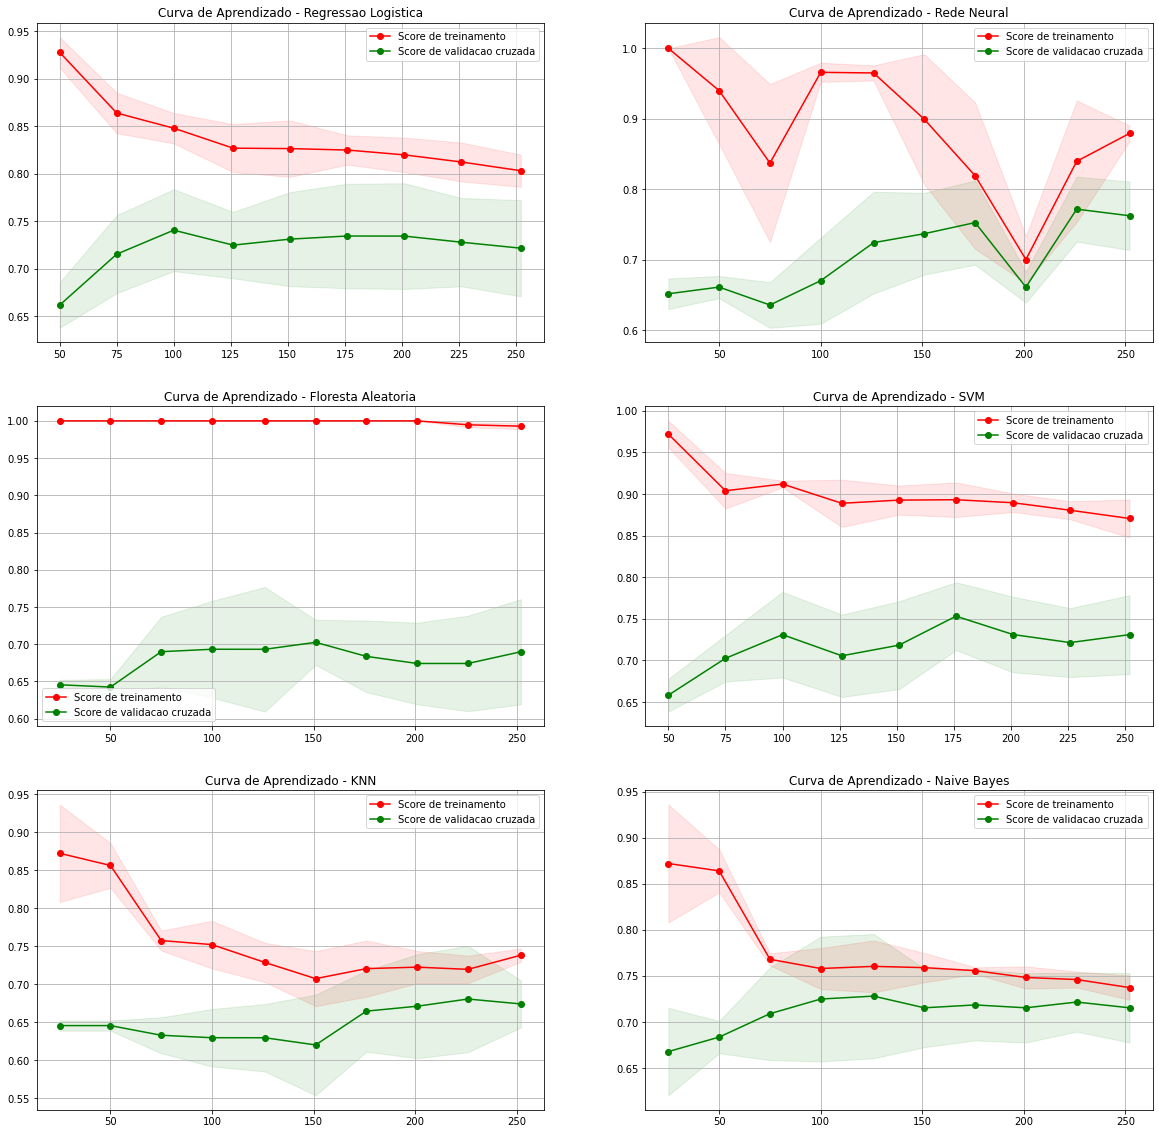
\includegraphics[width=.45\textwidth]{curva.png}
  \caption{Curva de aprendizado dos classificadores}
\label{fig:short}
\end{figure}

Ademais, como pode-se ver na tabela III, contendo os resultados do modelo com 72 atributos, observando os valores da curva ROC para os modelos citados anteriormente, confirma o bom desempenho destes 3 classificadores.

Por fim, os resultados de cada um dos 6 modelos de classificação no placar público da competição no Kaggle pode ser visto na tabela IV.

\begin{table}[]
\caption{Métricas dos algoritmos para a base com 72 atributos}
\centering
\resizebox{\columnwidth}{!}{%
\begin{tabular}{|c|c|}
\hline
Classificador & Pontuação (Placar Público Kaggle)\\ \hline
KNN           & 0.5   \\ \hline
Naive Bayes   & 0.7   \\ \hline
Regressão Logistica & 0.75 \\ \hline
Rede Neural Artificial & 0.725 \\ \hline
Máquina de Vetores de Suporte & 0.55 \\ \hline
Floresta Aleatoria & 0.625 \\ \hline
\end{tabular}%
}
\end{table}

\section{Estratégia Final}
A solução final escolhida para envio na competição foram dos métodos de Regressão Logística, apresentou 75\% de pontuação no placar público da competição no Kaggle, e Rede Neural Artificial, apresentou 72,5\% de pontuação.

\subsection{Base de dados}
A base de dados após todos os pré-processamentos, e escolha final de atributos selecionados, por parte do método de seleção, ficou contida com 72 atributos, sendo 2 atributos clínicos, 55 atributos de mutação gênica e 15 atributos de expressão genética. Sendo que os atributos foram os seguintes:

- Clínicos: Diagnosis Age e ELN Risk Classification.

- Expressão Genética: OSBPL5, DDIT4, LTK, EXT2, SLC29A2, CALR, CERCAM, AGRN, H2AFY, ECE1, GALNT1, PPM1H, MICALL2, SLC25A29 e LPPR3.

- Mutação Gênica: FLT3, TP53, U2AF1, PHF6, CALR, THRAP3, PHIP, PKD1L2, CADM2, BICD1, C5, CAPN6, CSF3R, CTNNA2, DIAPH2, DOCK1, EPHB1, HSPA4, KCNJ6, LTBP3, MAX, PKNOX1, PLRG1, PRKAA2, SRSF2, SLC4A3, SOX5, KMT2D, CACNA1G, SLC7A7, AURKB, DDX23, CEP170, ATP6AP2, POSTN, ATG14, MYH15, IGSF9B, GPATCH8, DOCK9, ATRNL1, FILIP1, PCDH11X, SETD2, THEG, LIMA1, NECAB2, PARP14, RIF1, ELMOD1, RALGAPA2, PAPPA2, ARHGEF28, WNK4 e KIAA1109.

\subsection{Melhores Parâmetros}
Os parâmetros dos métodos de classificação também foram testados de forma a buscar o qual proporciona melhor desempenho do modelo, dessa forma, para os modelos escolhidos, obteve-se “hidden\_layer\_sizes”, o i-ésimo elemento representa o número de neurônios na i-ésima camada oculta, com valor de (10, 10) para Rede Neural Artificial, e para o método de Regressão Logística o parâmetro “C”,  inverso da força de regularização, com valor 1, os demais parâmetros escolhidos para os outros métodos podem ser vistos na tabela V.

\begin{table}[]
\caption{Melhores Parâmetros para os métodos}
\centering
\resizebox{\columnwidth}{!}{%
\begin{tabular}{|c|c|c|c|c|c|}
\hline
Classificador & Melhores Parâmetros\\ \hline
KNN           & n\_neighbors: 17   \\ \hline
Naive Bayes   & var\_smoothing: 0.01   \\ \hline
Regressão Logistica & C: 1 \\ \hline
Rede Neural Artificial & hidden\_layer\_sizes: (10, 10) \\ \hline
Máquina de Vetores de Suporte & C: 1000 \\ \hline
Floresta Aleatoria & n\_estimators: 100 \\ \hline
\end{tabular}%
}
\end{table}

\section{Conclusão}
Conclui-se que o sistema de auxílio na predição de desfecho clínico apresenta resultados promissores na ajuda da indicação de melhores tratamentos para os pacientes no contexto da Leucemia Mieloide Aguda, mostrando-se um campo sujeito a maior exploração no âmbito médico, visto que os métodos de aprendizado de máquina mostram-se capazes de encontrar relações e padrões tal como este trabalho demonstrou. Ademais, os resultados obtidos são satisfatórios, mas apresentam um horizonte para extrair melhorias em diversos fatores, realizando-se um maior aprofundamento do que foi abordado. Dessa forma, o sistema pode ser adotado como mais uma ferramenta no auxílio de predição de tratamentos médicos para LMA, acompanhada de um especialista validando a utilidade das informações.

% conference papers do not normally have an appendix


\begin{thebibliography}{1}

\bibitem{}
YU, X. et al. Predicting lung adenocarcinoma disease progression using methylationcorrelated blocks and ensemble machine learning classifiers. PeerJ, v. 9, p. e10884–e10884, 2021.

\bibitem{}
ARBER, D. A. et al. International Consensus Classification of Myeloid Neoplasms and Acute Leukemias: integrating morphologic, clinical, and genomic data. Blood, v. 140, n. 11, p. 1200–1228, 2022.

\bibitem{}
CAMPOS, m. g., OLIVEIRA, j. s., CHAUFAILLE, m. l. (2006). Considerações sobre idade e perfil de apresentação em leucemia mielóide crônica. Revista Brasileira de Hematologia Hemoter, 28(Supl.2): Abstr.452. 

\bibitem{}
DO CARMO, c. s., TEIXEIRA, j. r., TEIXEIRA, j. (2014). Leucemia- sociedade em riscos. 

\bibitem{}
MEIRELES, m. f., PAIVA, g. p. (2017). leucemia mieloide. rev brasileira , 12-25

\end{thebibliography}


% that's all folks
\end{document}